\documentclass{article}
\usepackage{PreambleCommon}
\usepackage{minted}
\usepackage[vlined, ruled, linesnumbered]{algorithm2e}


\title{Assignment 10: Graph DFS With Stacks/Iteration \\[8pt] CS3305/W01 Data Structures}
\author{Casey Hampson}

\begin{document}
\maketitle

\section*{Pseudocode/Algorithm}
We can take inspiration from the small listing in the Checkpoint Question 28.17. The thing that is wrong in that listing is that there is the possibility that we can visit the starting vertex twice. This happens because we push the starting vertex $v$ onto the stack, then we pop it back off, visit it again, and continue going. Instead, we should only visit vertices that we search out from given some vertex that we pop. So:

\begin{algorithm}[H]
  \SetKwInOut{Input}{input}\SetKwInOut{Output}{output}
  
  \Input{Vertex $v$}
  \BlankLine
  push v onto the stack\;
  \BlankLine
  \While{the stack is not empty}{
    pop a vertex $u$ from the stack\;
    \BlankLine
    \For{each neighber $n$ of $u$}{
      \If{$n$ has not been visited}{
        add $n$ to the stack and search order array\;
        store $w$ as the parent of $n$\;
      }
    }
  }
\end{algorithm}

With this, we still push the first vertex onto the stack only to immediately pop it back off, but by only ``visiting'' the vertices during the iteration of the popped vertex's neighbors, we eliminate any double counting issue.



\section*{Program Output}
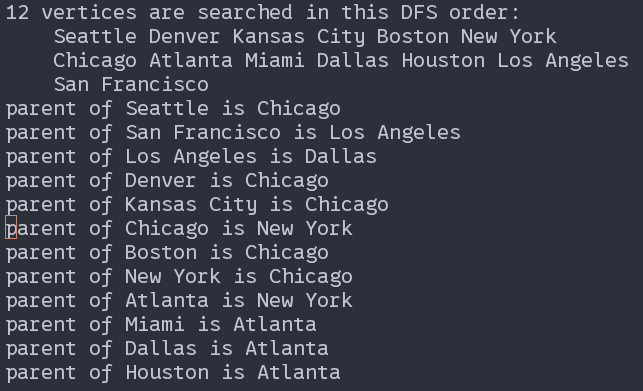
\includegraphics[width=0.8\linewidth]{./res/1.png}


\pagebreak
\section*{Source Code}
\inputminted{java}{./A10.java} 




\end{document}

%%% Local Variables:
%%% mode: LaTeX
%%% TeX-master: t
%%% End:
